% Four block structures of a variational circuit on N = 8 qubits (notebook 42a, Section 5.1).
% Every white box is a parametrised unitary on the wires it covers; boxes joined by a line act on non-adjacent wires.
% (a) tree tensor network: root on (0,4), then (0,2),(4,6), then (0,1),(2,3),(4,5),(6,7)
% (b) matrix-product (staircase): (0,1),(1,2),...,(6,7)
% (c) alternating layers, two-fold: even bonds, odd bonds, repeated (block_ansatz with brick_bonds)
% (d) alternating layers, three-fold: three-qubit blocks shifted by one wire per column
\documentclass[tikz,border=6pt]{standalone}
\usepackage{amsmath,amssymb}
\usetikzlibrary{positioning,calc}
\newcommand{\wires}[2]{\foreach \q in {0,...,7} {\draw[thick] (#1,-0.55*\q) -- (#2,-0.55*\q);}}
% block from wire #2 to wire #3 at horizontal position #1
\newcommand{\blk}[3]{\draw[thick, fill=white] (#1-0.27,-0.55*#2+0.21) rectangle (#1+0.27,-0.55*#3-0.21);}
% two-qubit block on non-adjacent wires #2 and #3
\newcommand{\lnk}[3]{\draw[thick] (#1,-0.55*#2) -- (#1,-0.55*#3);
  \draw[thick, fill=white] (#1-0.27,-0.55*#2+0.21) rectangle (#1+0.27,-0.55*#2-0.21);
  \draw[thick, fill=white] (#1-0.27,-0.55*#3+0.21) rectangle (#1+0.27,-0.55*#3-0.21);}
\begin{document}
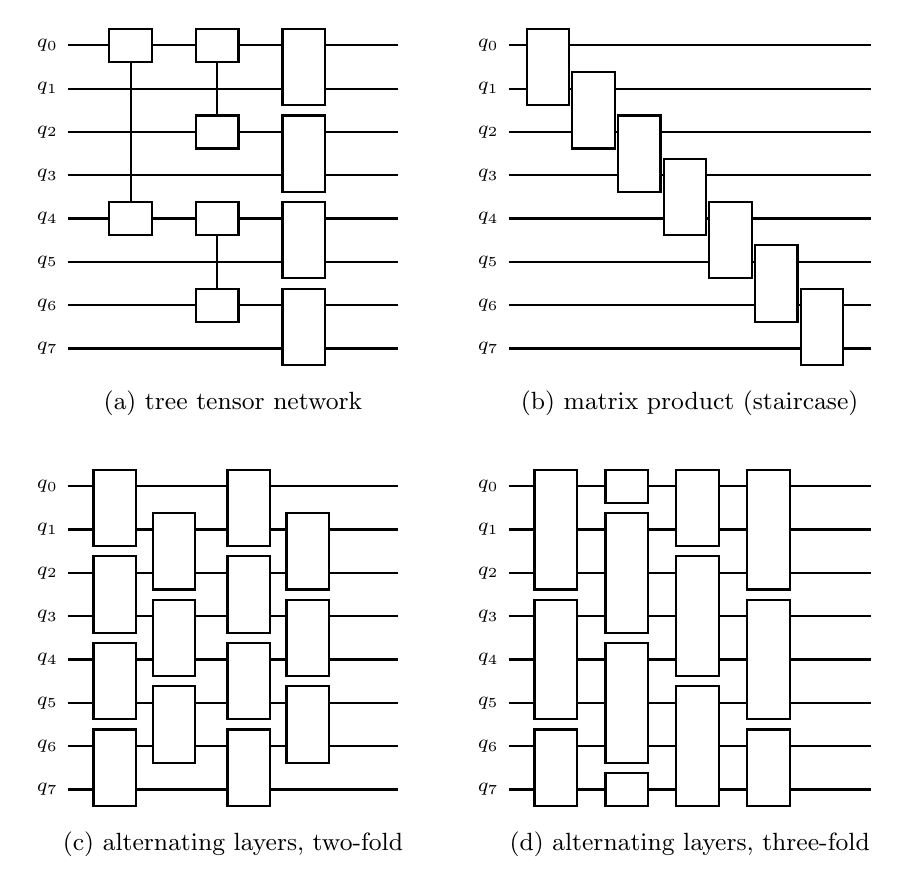
\begin{tikzpicture}
  % ------------------------------------------------------------------ (a) tree
  \begin{scope}[shift={(0,0)}]
    \wires{0}{4.2}
    \foreach \q in {0,...,7} {\node[anchor=east, font=\scriptsize] at (0,-0.55*\q) {$q_{\q}$};}
    \lnk{0.8}{0}{4}
    \lnk{1.9}{0}{2} \lnk{1.9}{4}{6}
    \blk{3.0}{0}{1} \blk{3.0}{2}{3} \blk{3.0}{4}{5} \blk{3.0}{6}{7}
    \node[font=\small] at (2.1,-4.55) {(a) tree tensor network};
  \end{scope}
  % ------------------------------------------------------------------ (b) staircase
  \begin{scope}[shift={(5.6,0)}]
    \wires{0}{4.6}
    \foreach \q in {0,...,7} {\node[anchor=east, font=\scriptsize] at (0,-0.55*\q) {$q_{\q}$};}
    \foreach \q in {0,...,6} {\blk{0.5+0.58*\q}{\q}{\the\numexpr\q+1\relax}}
    \node[font=\small] at (2.3,-4.55) {(b) matrix product (staircase)};
  \end{scope}
  % ------------------------------------------------------------------ (c) two-fold alternation
  \begin{scope}[shift={(0,-5.6)}]
    \wires{0}{4.2}
    \foreach \q in {0,...,7} {\node[anchor=east, font=\scriptsize] at (0,-0.55*\q) {$q_{\q}$};}
    \foreach \x in {0.6,2.3} {
      \foreach \q in {0,2,4,6} {\blk{\x}{\q}{\the\numexpr\q+1\relax}}
      \foreach \q in {1,3,5} {\blk{\x+0.75}{\q}{\the\numexpr\q+1\relax}}
    }
    \node[font=\small] at (2.1,-4.55) {(c) alternating layers, two-fold};
  \end{scope}
  % ------------------------------------------------------------------ (d) three-fold alternation
  \begin{scope}[shift={(5.6,-5.6)}]
    \wires{0}{4.6}
    \foreach \q in {0,...,7} {\node[anchor=east, font=\scriptsize] at (0,-0.55*\q) {$q_{\q}$};}
    \blk{0.6}{0}{2} \blk{0.6}{3}{5} \blk{0.6}{6}{7}
    \blk{1.5}{0}{0} \blk{1.5}{1}{3} \blk{1.5}{4}{6} \blk{1.5}{7}{7}
    \blk{2.4}{0}{1} \blk{2.4}{2}{4} \blk{2.4}{5}{7}
    \blk{3.3}{0}{2} \blk{3.3}{3}{5} \blk{3.3}{6}{7}
    \node[font=\small] at (2.3,-4.55) {(d) alternating layers, three-fold};
  \end{scope}
\end{tikzpicture}
\end{document}
